% Based on Model 2 of "Activity 01 - Operators" by Helen Hu

\model{The \% Operator}

\vspace{-1ex}
\begin{center}
\begin{tabular}[t]{|C{35pt}|C{65pt}|C{35pt}|}
\hline
 9 / 4 & \textit{evaluates to} & 2 \\
\hline
10 / 4 & \textit{evaluates to} & 2 \\
\hline
11 / 4 & \textit{evaluates to} & 2 \\
\hline
12 / 4 & \textit{evaluates to} & 3 \\
\hline
13 / 4 & \textit{evaluates to} & 3 \\
\hline
14 / 4 & \textit{evaluates to} & 3 \\
\hline
15 / 4 & \textit{evaluates to} & 3 \\
\hline
16 / 4 & \textit{evaluates to} & 4 \\
\hline
\end{tabular}
\hspace{0.5in}
\begin{tabular}[t]{|C{35pt}|C{65pt}|C{35pt}|}
\hline
 9 \% 4 & \textit{evaluates to} & 1 \\
\hline
10 \% 4 & \textit{evaluates to} & 2 \\
\hline
11 \% 4 & \textit{evaluates to} & 3 \\
\hline
12 \% 4 & \textit{evaluates to} & 0 \\
\hline
13 \% 4 & \textit{evaluates to} & 1 \\
\hline
14 \% 4 & \textit{evaluates to} & 2 \\
\hline
15 \% 4 & \textit{evaluates to} & 3 \\
\hline
16 \% 4 & \textit{evaluates to} & 0 \\
\hline
\end{tabular}
\end{center}


\quest{12 min}


\Q Which numbers \% 4 evaluate to 0 in the table above?
If the table were extended to include more rows, which other numbers \% 4 would evaluate to 0?

\begin{answer}
12 and 16. Other numbers include 0, 4, 8, 20, 24.
\end{answer}


\Q Look at the expressions in the second table that evaluate to 1.
How do the left operands in these expressions (9, 13, 17) differ from those that evaluate to 0?

\begin{answer}
They differ by one.
\end{answer}


\Q List three numbers \% 5 that will evaluate to 0 and three numbers \% 5 that will evaluate to 2.

\begin{answer}
0, 5, 10 and 2, 7, 12.
\end{answer}


\Q Evaluate the following Java expressions:

\begin{center}
\begin{tabular}{C{1in}C{1in}C{1in}C{1in}}
18 \% 4 \ans{= ~2} &
19 \% 4 \ans{= ~3} &
19 \% 5 \ans{= ~4} &
19 \% 6 \ans{= ~1} \\
\end{tabular}
\end{center}


\newpage

\Q Consider how you were taught to do long division in elementary school.
Finish solving for $79 \div 5$.
What is the answer?

\begin{center}
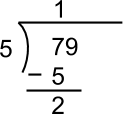
\includegraphics[scale=0.65]{div79by5.png}
\end{center}

\begin{answer}[3em]
We first bring the 9 down, then 5 goes into 29 five times, and so we subtract 25. The final answer is 15 remainder 4.
\end{answer}


\Q \label{mints}
Imagine that you are given candy mints to divide evenly among your team members.

\begin{enumerate}
\item If your team receives 11 mints, how many mints are left over?

\ans{\java{11 \% 4} is 3 ~~or~~ \java{11 \% 5} is 1}

\item If your team receives 2 mints, how many mints are left over?

\ans{\java{2 \% 4} is 2 ~~or~~ \java{2 \% 5} is 2}
\end{enumerate}


\Q \label{modoper}
Describe what the \% operator does.
How are the / and \% operators related?

\begin{answer}
Both operators divide two numbers: \% returns the remainder, and / returns the quotient.
\end{answer}


\Q \label{modreal}
Would it make sense to apply the \% operator to real numbers?
Why or why not?

\begin{answer}
Not really, since the concept of remainder is based on integer division.

(BTW floating-point modulo is defined in IEEE 754, but its use is rare.)
\end{answer}
